\documentclass[a4paper,12pt]{article}
\usepackage[a4paper,top=1.3cm,bottom=2cm,left=1.5cm,right=1.5cm,marginparwidth=0.75cm]{geometry}

% Пакеты
\usepackage{mathtext} 
\usepackage{setspace}
\usepackage{tabularx}
\usepackage{cmap}
\usepackage{longtable}
\usepackage{icomma}
\usepackage{euscript}
\usepackage{float}
\usepackage{cutwin}
\usepackage{mathrsfs}
\usepackage{adjustbox}
\usepackage{dashbox}
\usepackage[normalem]{ulem}
\usepackage[T2A]{fontenc}			
\usepackage[utf8]{inputenc}                 %!  закрепляет кодировку utf8
\usepackage[english,russian]{babel}         %!  подключает русский и английский
%математические шрифты:
\usepackage{amsmath,amsfonts,amssymb,amsthm,mathrsfs,mathtools} 
\usepackage[colorlinks, linkcolor = purple]{hyperref}      %!  оглавление для панели навигации по PDF-документу + гиперссылки
\usepackage{xcolor}                         %!  добавляет цвета
\usepackage{enumitem}                       %!  задание макета перечня.
\usepackage{xpatch}                         %?  работа с renewcommand и макросами              
\usepackage{cancel}                         %   зачёкивания текста (!!!) для slash-нотации использовать \usepackage{slashed}!!
\usepackage{upgreek}                        %   заглавные греческие буквы
\usepackage{lipsum}                         %?  для вставки кучи текста при форматировании
\usepackage[version=4]{mhchem}              %   химические формулы
\usepackage{multirow}                       %   объединение строк в матрицах
\usepackage{stackengine}                    %   stack символов
\usepackage{tikz}                           %!  рисунки
\usetikzlibrary{positioning}                %?  библиотека для тикза 
\usepackage{titletoc}                       %!  форматирование содержания и заголовков
\usepackage{titlesec}                       %!  форматирование содержания и заголовков
\usepackage{wrapfig}                        %   обтекание таблиц и рисунков
\usepackage{chngcntr}                       %!  для setcounter
\usepackage{fancyhdr}                       %!  для колонтитулов
\usepackage{makecell}                       %?  матрицы с разными выравниваниями и т.п
\usepackage{indentfirst}                    %   добавить indent перед первым 
\usepackage{tocloft}                        %?  изменение названий глав и разделов                       
\usepackage{soul}                           %   типографические примочки, типо зачёркивания и подчёркивания
\usepackage[stable]{footmisc}               %?  продвинутые сноски
\usepackage{subfig}                         %   несколько картинок рядом
%  задаёт поля страниц

% pgf plots
% \usepackage{pgfplots}
% \pgfplotsset{compat=1.17}

\mathtoolsset{showonlyrefs=true}

%Обозначения теорем и т.п
\theoremstyle{definition}
\newtheorem*{definition}{Определение}
\newtheorem{statement}{Предложение}[section]
\newtheorem{lemma}{Лемма}[section]
\newtheorem{theorem}{Теорема}[section]
\newtheorem*{theoremn}{Теорема}
\newtheorem*{corollary}{Следствие}
\newtheorem*{example}{Пример}
\newtheorem*{note}{Замечание}
\newtheorem*{problem}{Задача}

%Шарабара для содержания и внешнего вида нумерации
\counterwithout{footnote}{section}\DeclareRobustCommand{\divby}{%
	\mathrel{\text{\vbox{\baselineskip.65ex\lineskiplimit0pt\hbox{.}\hbox{.}\hbox{.}}}}%
}



%Толерантный квадратик чтд
%\makeatletter \renewenvironment{proof}[1][\proofname]{\par\pushQED{\qed}\normalfont\topsep6\p@\@plus6\p@\relax\trivlist\item[\hskip\labelsep\bfseries#1\@addpunct{.}]\ignorespaces}{\popQED\endtrivlist\@endpefalse} \makeatother
%\renewcommand\qedsymbol{$\squareulblack$}
%\newcommand{\usubseteq}{\mathbin{\rotatebox[origin=c]{90}{$\subset$}}}
%\DeclareFontEncoding{LS2}{}{\noaccents@}
%\DeclareFontSubstitution{LS2}{stix}{m}{n}
%\DeclareSymbolFont{arrows3}{LS2}{stixtt}{m}{n}
%\DeclareMathSymbol{\squareulblack}{\mathord}{arrows3}{"88}

%Разные операторы и символы
\newcommand{\dotpr}[2]{\bra{#1}\ket{#2}}
\let\AA\relax
%\let\oldvarphi\phi %оно делает так, что \phi становится правильным фи
%\let\phi\varphi
%\let\varphi\oldvarphi
\let\emptyset\varnothing
\DeclareMathOperator*{\esssup}{ess sup}
\DeclareMathOperator*{\ord}{ord}
\DeclareMathOperator*{\supp}{supp}
\DeclareMathOperator*{\pr}{pr}
\DeclareMathOperator*{\Ker}{Ker}
\DeclareMathOperator*{\Vol}{Vol}
\DeclareMathOperator*{\rg}{rk}
\DeclareMathOperator*{\Ima}{Im}
\DeclareMathOperator*{\Alt}{Alt}
\DeclareMathOperator*{\Sym}{Sym}
\newcommand{\eqdef}{\stackrel{\text{\tiny{def}}}{=}}
\newcommand{\pp}{\partial}
\newcommand{\AA}{\mathcal{A}}
\newcommand{\BB}{\mathcal{B}}
\newcommand{\MM}{\mathbb{M}}
\newcommand{\NN}{\mathbb{N}}
\newcommand{\ZZ}{\mathbb{Z}}
\newcommand{\QQ}{\mathbb{Q}}
\newcommand{\RR}{\mathbb{R}}
\newcommand{\CC}{\mathbb{C}}
\newcommand{\FFF}{\mathbb{F}}
\newcommand{\DD}{\mathcal{D}}
\newcommand{\FF}{\mathcal{F}}
\newcommand{\sS}{\mathcal{S}}
\newcommand*\circled[1]{\tikz[baseline=(char.base)]{
		\node[shape=circle,draw,inner sep=2pt] (char) {#1};}}

\title{Измерение вязкости воздуха по течению в тонких трубках (1.3.3)}
\author{Павлушкин Вячеслав}
\date{\today}


\begin{document}
	\maketitle
	\section{Аннотация}
	В данной работе проводится экспериментальное выявление участка сформировавшегося ламинарного течения; экспериментально определяются режимы ламинарного и турбулентного течения; проводится определение числа Рейнольдса.
	
	\section{Введение}
	
	\noindent\textbf{Цель работы:} экспериментально исследовать свойства течения газов по тонким трубкам при различных числах Рейнольдса; выявить область применимости закона Пуазейля и с его помощью определить коэффициент вязкости воздуха.
	
	
	\bigskip
	\noindent\textbf{В работе используются:} система подачи воздуха (компрессор, поводящие трубки); газовый счетчик барабанного типа; спиртовой микроманометр с регулируемым наклоном; набор трубок различного диаметра с выходами для подсоединения микроманометра; секундомер
		
	\section{Теоретические сведения}
	Характер движения газа по трубке определяется числом Рейнольдса:
	\begin{equation}
		Re = \frac{u r \rho}{\eta},
		\label{eq:Re}
	\end{equation}
	где $u$ - скорость потока, $r$ - радиус трубки, $\rho$ - плотность жидкости, $\eta$ - вязкость. Переход от ламинарного движения к турбулентному: $Re \sim 1000$.
	
	Для ламинарного течения при постоянном удельном объеме верна формула Пуазейля:
	\begin{equation}
		Q_V = \frac{\pi r^4}{8 l \eta}(P_1 - P_2),
		\label{eq:Pu}
	\end{equation}
	где $P_1 - P_2$ - разность давлений в двух сечениях, расстояние между которыми - $l$. Формула позволяет определить вязкость по расходу $Q_V$.
	
	Ламинарное течение газа устанавливается на расстоянии
	\begin{equation}
		a \sim 0.2 r \cdot Re.
		\label{eq:Aa}
	\end{equation}
	Градиент давления на участке с турбулентным течением больше, чем на участке с ламинарным, что позволяет разделить их экспериментально.
	
	\section{Ход работы}
	
	В работе использовались 3 трубки, диаметрами: $d_1 = (3.0\pm0.1)$ мм, $d_2 = (3.95\pm0.05)$ мм, $d_3 = (5.05\pm0.0.5)$ мм.
	
	Для каждой трубки снимем зависимость $Q(\Delta P),$ с помощью секундомера и газового счетчика ($\sigma_v = 0.05\text{ Дц}^3$/м) получим расход, с помощью микроманометра -- разность давления на участке трубы ($\sigma_{\Delta P} = 0,5$ Дел. $ = 0.1$ Па).
	
	Проведем эксперимент для каждой трубы, на участке с наибольшей длиной, и получим таблицы:
	
	\begin{table}[H]
		\bgroup
		\def\arraystretch{1.0}%
		\centering
		\begin{minipage}{.49\linewidth}
			\centering
			\begin{tabular}{|c|c|c|c|}
				\hline
				\multicolumn{4}{|c|}{$d_2$ = 3.95 мм }\\ \hline
				$V$, $\text{Дц}^3$& $t,$ с&$\Delta P,$ Дел.  & $Q\cdot 10^{-6},$ $\text{м}^3$/с\\ \hline
				0.3 & 86.45 & 3 & 3 \\ \hline
				0.5 & 38.61 & 10 & 13 \\ \hline
				0.5 & 20.49 & 19 & 24 \\ \hline
				1 & 28.04 & 28 & 36 \\ \hline
				1 & 20.60 & 39 & 49 \\ \hline
				1.5 & 24.06 & 49 & 62 \\ \hline
				2 & 27.26 & 60 & 73 \\ \hline \hline
				2 & 24.14 & 68 & 83 \\ \hline
				2 & 21.12 & 82 & 95 \\ \hline
				2.5 & 24.66 & 91 & 101 \\ \hline
				2.5 & 23.68 & 102 & 106 \\ \hline
				2.5 & 23.15 & 113 & 108 \\ \hline
				2.5 & 23.02 & 131 & 109 \\ \hline
				2.5 & 19.52 & 180 & 128 \\ \hline
				4 & 26.21 & 250 & 153 \\ \hline
			\end{tabular}
		\end{minipage}
		\begin{minipage}{.49\linewidth}
			\centering
			\begin{tabular}{|c|c|c|c|}
				\hline
				\multicolumn{4}{|c|}{$d_3$ = 5.05 мм }\\ \hline
				$V$, $\text{Дц}^3$& $t,$ с&$\Delta P,$ Дел.  & $Q\cdot 10^{-6},$ $\text{м}^3$/с\\ \hline
				1 & 35.29 & 7 & 28 \\ \hline
				1.5 & 27.98 & 14 & 54 \\ \hline
				1.5 & 22.98 & 18 & 65 \\ \hline
				2 & 25.65 & 20 & 78 \\ \hline
				2 & 20.13 & 26 & 99 \\ \hline
				2.5 & 21.66 & 30 & 115 \\ \hline
				2.5 & 21.14 & 33 & 118 \\ \hline
				3 & 22.83 & 39 & 131 \\ \hline \hline
				3 & 22.15 & 42 & 135 \\ \hline
				3.5 & 22.40 & 61 & 156 \\ \hline
				3.5 & 20.35 & 78 & 172 \\ \hline
				4 & 19.77 & 103 & 202 \\ \hline
				5 & 21.84 & 130 & 229 \\ \hline
				5.5 & 21.79 & 155 & 252 \\ \hline
				5.5 & 20.74 & 171 & 265 \\ \hline
			\end{tabular}
		\end{minipage}
		\egroup
		\caption{Результаты измерений двух трубок}
		\label{lowp}
	\end{table}  

	По полученным таблицам построим график $Q(\Delta P)$ по точкам на ламинарном участке (первые точки таблицы -- ламинарный поток, вторая половина -- турбулентный).
	
	\begin{figure}[H]
		\centering
		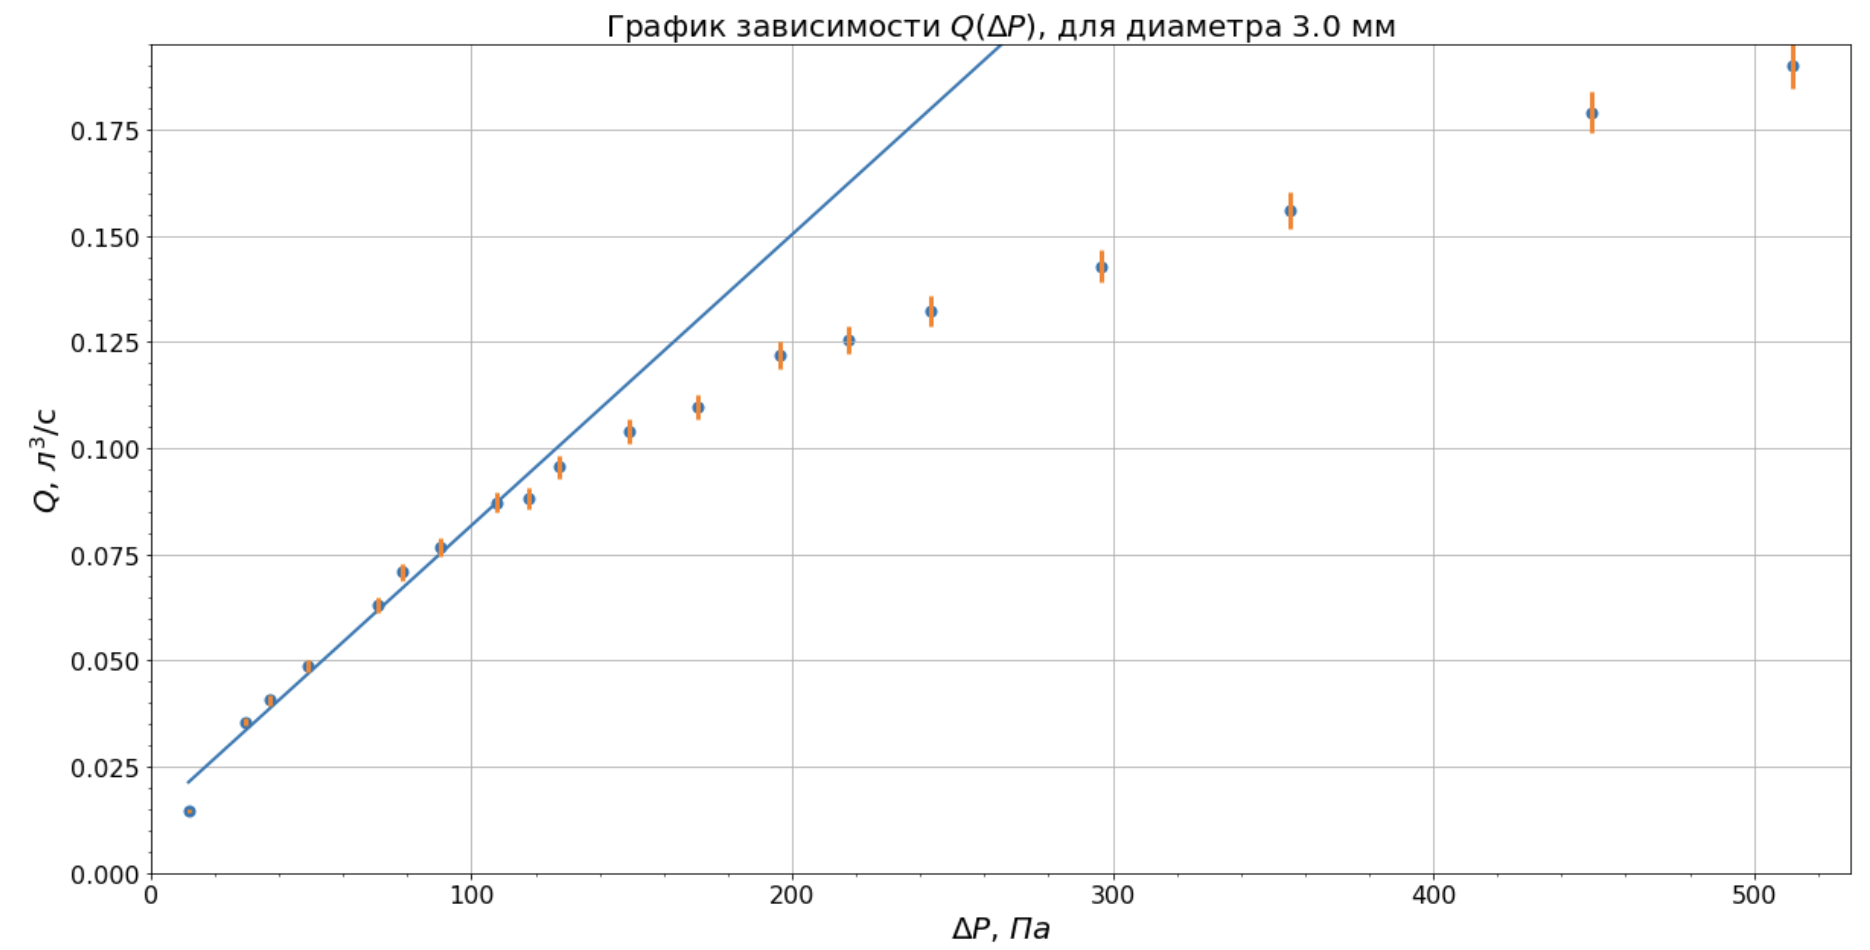
\includegraphics[scale = 0.5]{3.00}
		\caption{График зависимости $Q(\Delta P)$, для трубки диаметра 3.0 мм}
		\label{graph1}
	\end{figure}
	\begin{figure}[H]
		\centering
		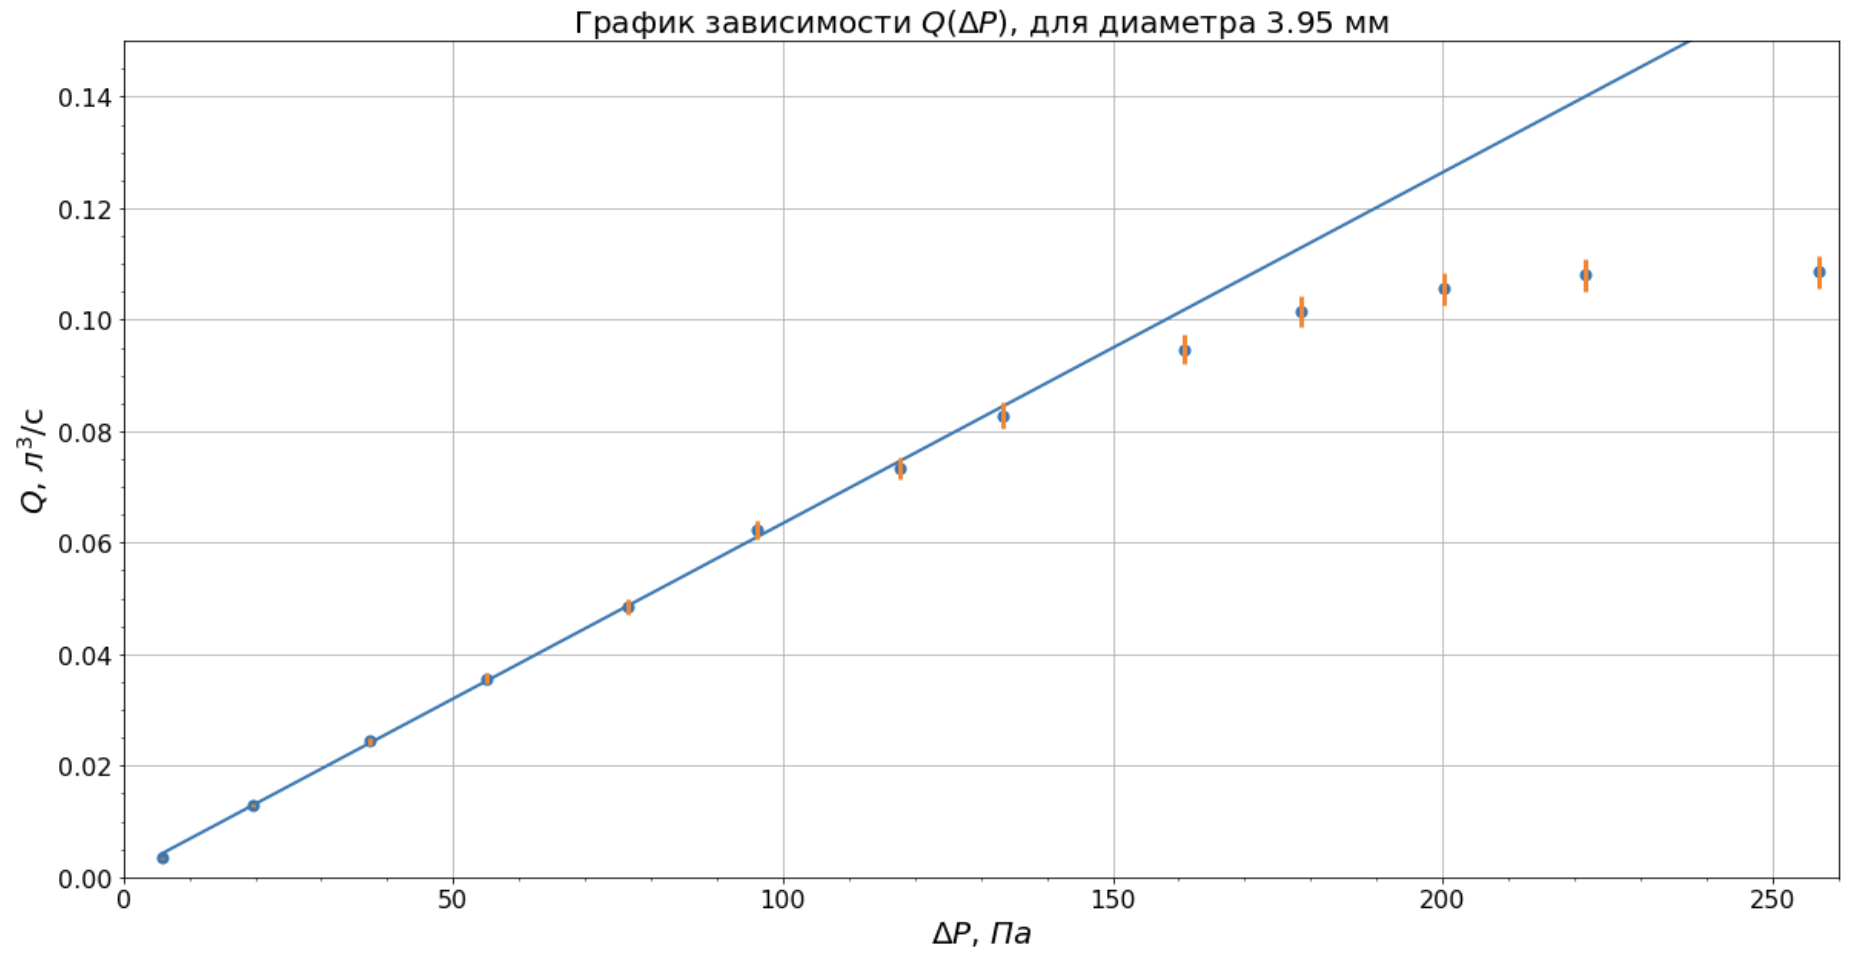
\includegraphics[scale = 0.55]{3.95}
		\caption{График зависимости $Q(\Delta P)$, для трубки диаметра 3.0 мм}
		\label{graph2}
	\end{figure}
	\begin{figure}[H]
		\centering
		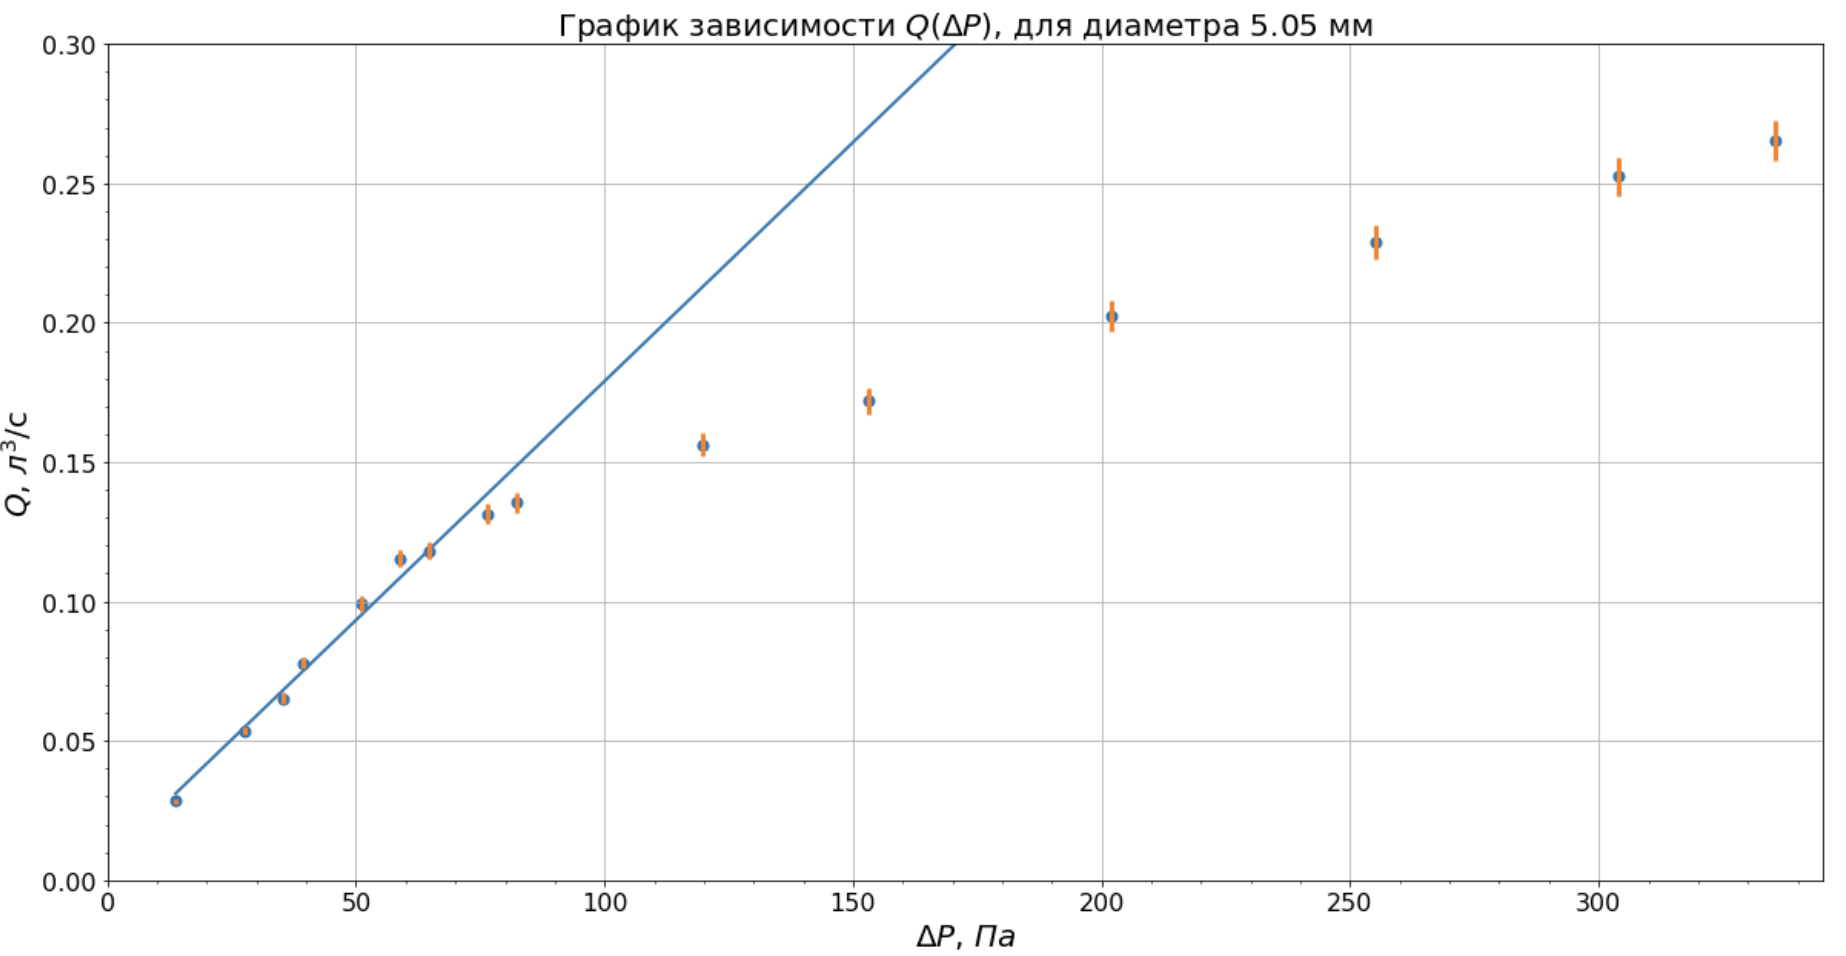
\includegraphics[scale = 0.55]{5.05}
		\caption{График зависимости $Q(\Delta P)$, для трубки диаметра 5.05 мм}
		\label{graph3}
	\end{figure}

	Линии проведены при помощи МНК, по точкам с ламинарным течением.
	
	С помощью коэффициентов наклона мы можем найти вязкость воздуха из формулы \eqref{eq:Re}:
	
	\begin{equation*}
		\eta = \frac{\pi R^4}{8kl}
	\end{equation*}
	где $k$ -- коэффициент наклона графика, $l$ -- длина участка трубы, а $R$ -- радиус трубки.
	
	По графикам определим значения коэффициента наклона с погрешностями:

	\begin{table}[H]
		\begin{center}
		\bgroup
		\def\arraystretch{1.1}%
			\begin{tabular}{|c|c|c|c|}
				\hline
				&$d_1 = 3.0$ мм&$d_2 = 3.95$ мм&$d_3 = 5.05$ мм\\ \hline
				$k\cdot10^{-7}$, $\text{м}^3$/с$\cdot$Па&6.85&6.29&17.14\\ \hline
				$\sigma_k^{\text{случ}}$, $\text{м}^3$/с$\cdot$Па&0.41&0.09&0.90\\ \hline
				$\sigma_k$, $\text{м}^3$/с$\cdot$Па&0.47& 0.22&1.06 \\ \hline
				$\eta\cdot10^{-5}$, Па$\cdot$с&1.45&1.89&1.86 \\ \hline
				$\sigma_\eta\cdot10^{-5}$, Па$\cdot$с&0.14&0.08&0.12\\ \hline
			\end{tabular}
		\egroup
		\caption{Результаты полученные из графиков}
		\label{highp}
		\end{center}
	\end{table}
	
	Заметно, что первое измерение достаточно сильно отличается от двух следующих, тогда возьмем, без учета первого диаметра:
	\begin{equation*}
		\eta = (1.88\pm 0.1) \text{ Па}\cdot \text{с}
	\end{equation*} 
	
	Далее найдем критическое число Рейнольдса $Re_\text{кр}$ для всех трубок:
	\begin{equation*}
		Re = \frac{\rho u R}{\eta} = \frac{\rho Q}{\pi R \eta}
	\end{equation*}
	\begin{itemize}
		\item $d_1 = 3.00$ мм: критический расход: $Q_1 = 91\cdot10^{-6}\text{ м}^3$/c, тогда $Re_1 = 1181 \pm 70.$
		\item $d_2 = 3.95$ мм: критический расход: $Q_2 = 78\cdot10^{-6}\text{ м}^3$/c, тогда $Re_2 = 763 \pm 40.$  
		\item $d_3 = 5.05$ мм: критический расход: $Q_3 = 131\cdot10^{-6}\text{ м}^3$/c, тогда $Re_3 =  1010\pm 45.$ 
	\end{itemize}

	Далее определим длину участка трубы, на котором происходит установление потока.
	
	Для этого построим графики зависимости $P(x)$ для каждой трубы.
	
	\begin{figure}[H]
		\centering
		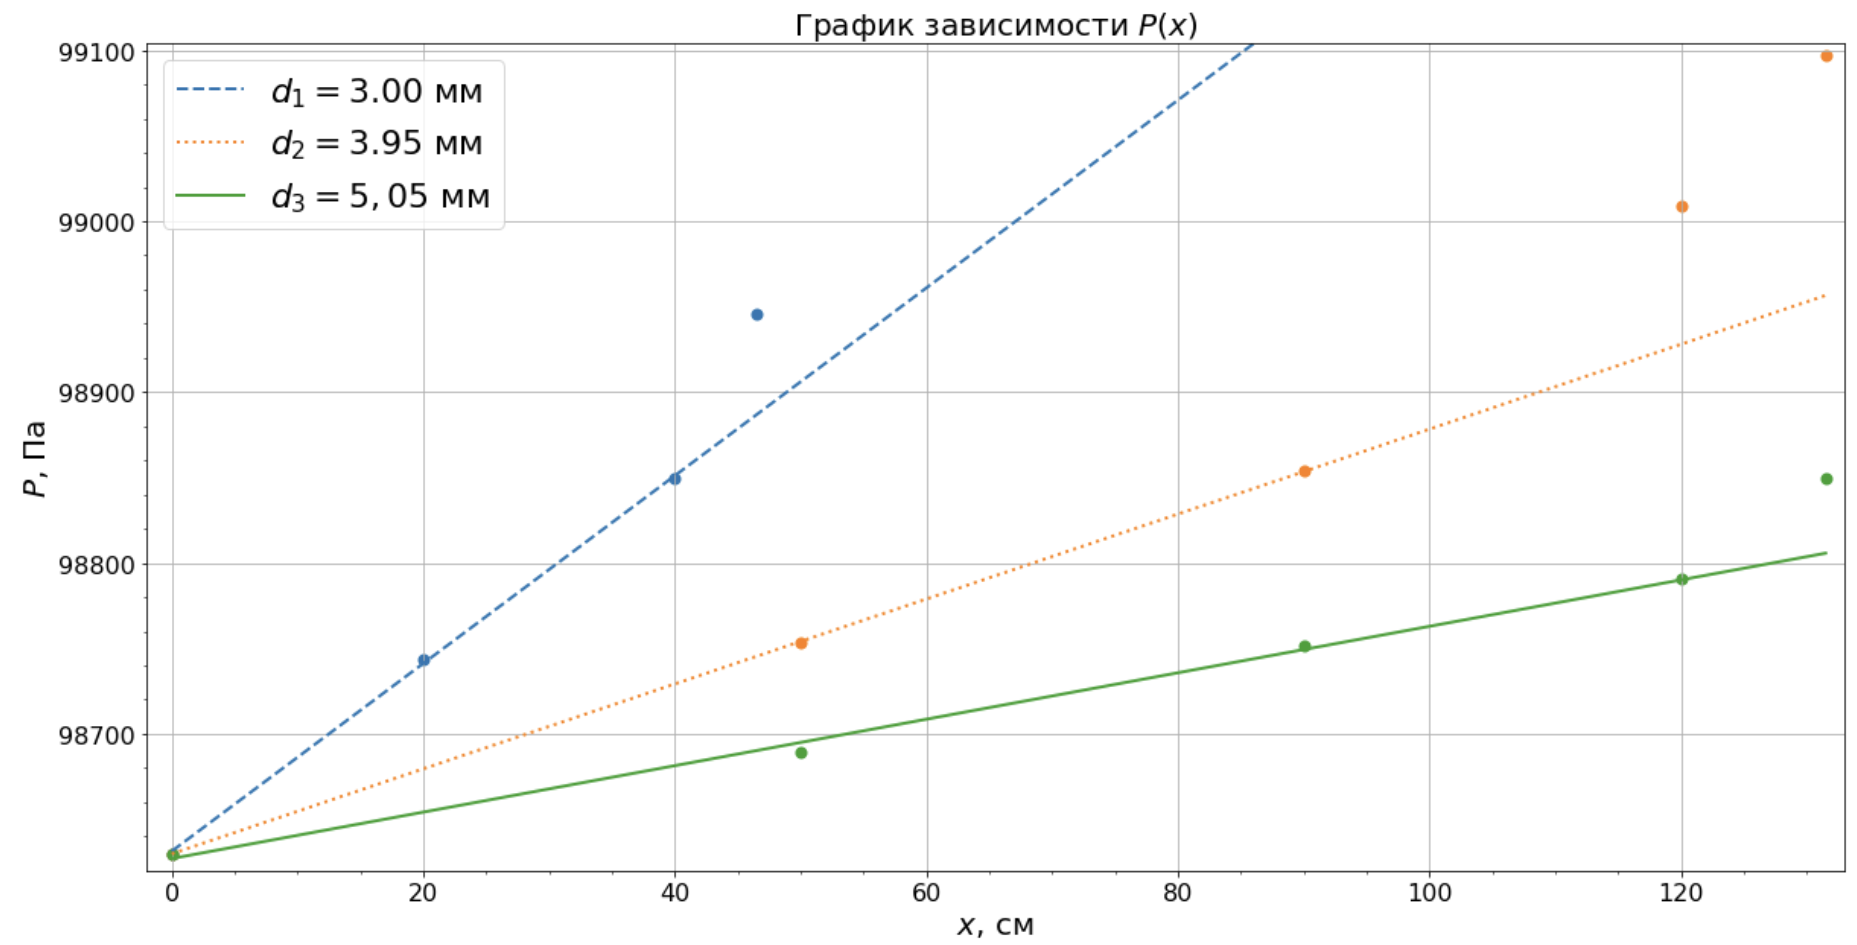
\includegraphics[scale = 0.55]{px}
		\caption{График зависимости $P(x)$}
		\label{graph4}
	\end{figure}

	По графику можно определить примерную длину участка, на котором устанавливается ламинарный поток (на графике отсчитывается от выхода трубы, я же рассматриваю длину на которой устанавливается поток, то есть от входа воздуха):
	\begin{itemize}
		\item $d_1 = 3.00$ мм, по графику поток устанавливается через 6.5 - 0 см от входа. По расчетам ($L_\text{уст} \approx 0.2R_1\cdot Re_1$)  получается 11.5 см. На мой взгляд полученный результат удовлетворительный.
		\item $d_2 = 3.95$ мм, по графику поток устанавливается через 41.5 - 0 см от входа. По расчетам ($L_\text{уст} \approx 0.2R_2\cdot Re_2$)  получается 30.1 см. Результат сходится с вычисленным.
		\item $d_3 = 5.05$ мм, по графику поток устанавливается через 41.5 - 0 см от входа. По расчетам ($L_\text{уст} \approx 0.2R_3\cdot Re_3$)  получается 51 см. Возможно, что формула примерная, поэтому я считаю, что данный результат тоже достаточно удовлетворительный.
	\end{itemize}

	Для проверки пропорциональности расхода к радиусу трубы при ламинарном и турбулентном режиме построим графики $\ln Q(\ln R)$ для разных труб при установившемся и неустановившемся течении.
	
	\begin{figure}[H]
		\centering
		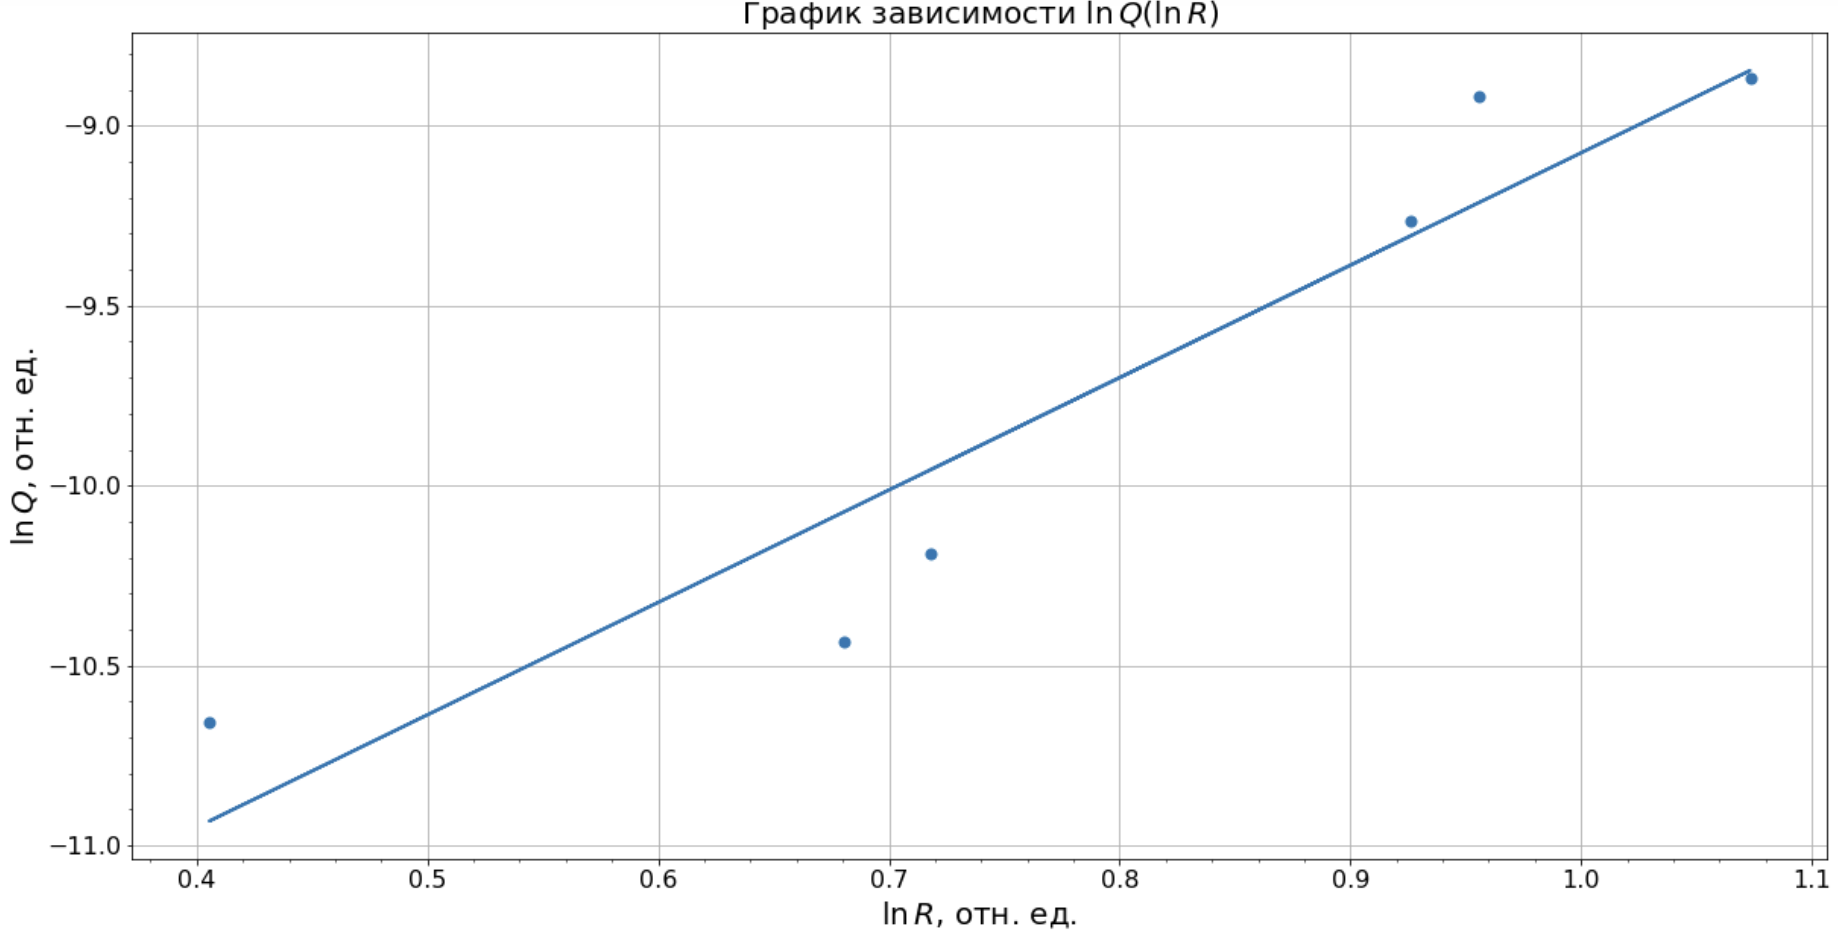
\includegraphics[scale = 0.5]{qr norm}
		\caption{График зависимости $P\ln Q(\ln R)$ для ламинарного течения}
		\label{graph5}
	\end{figure}

	\begin{figure}[H]
		\centering
		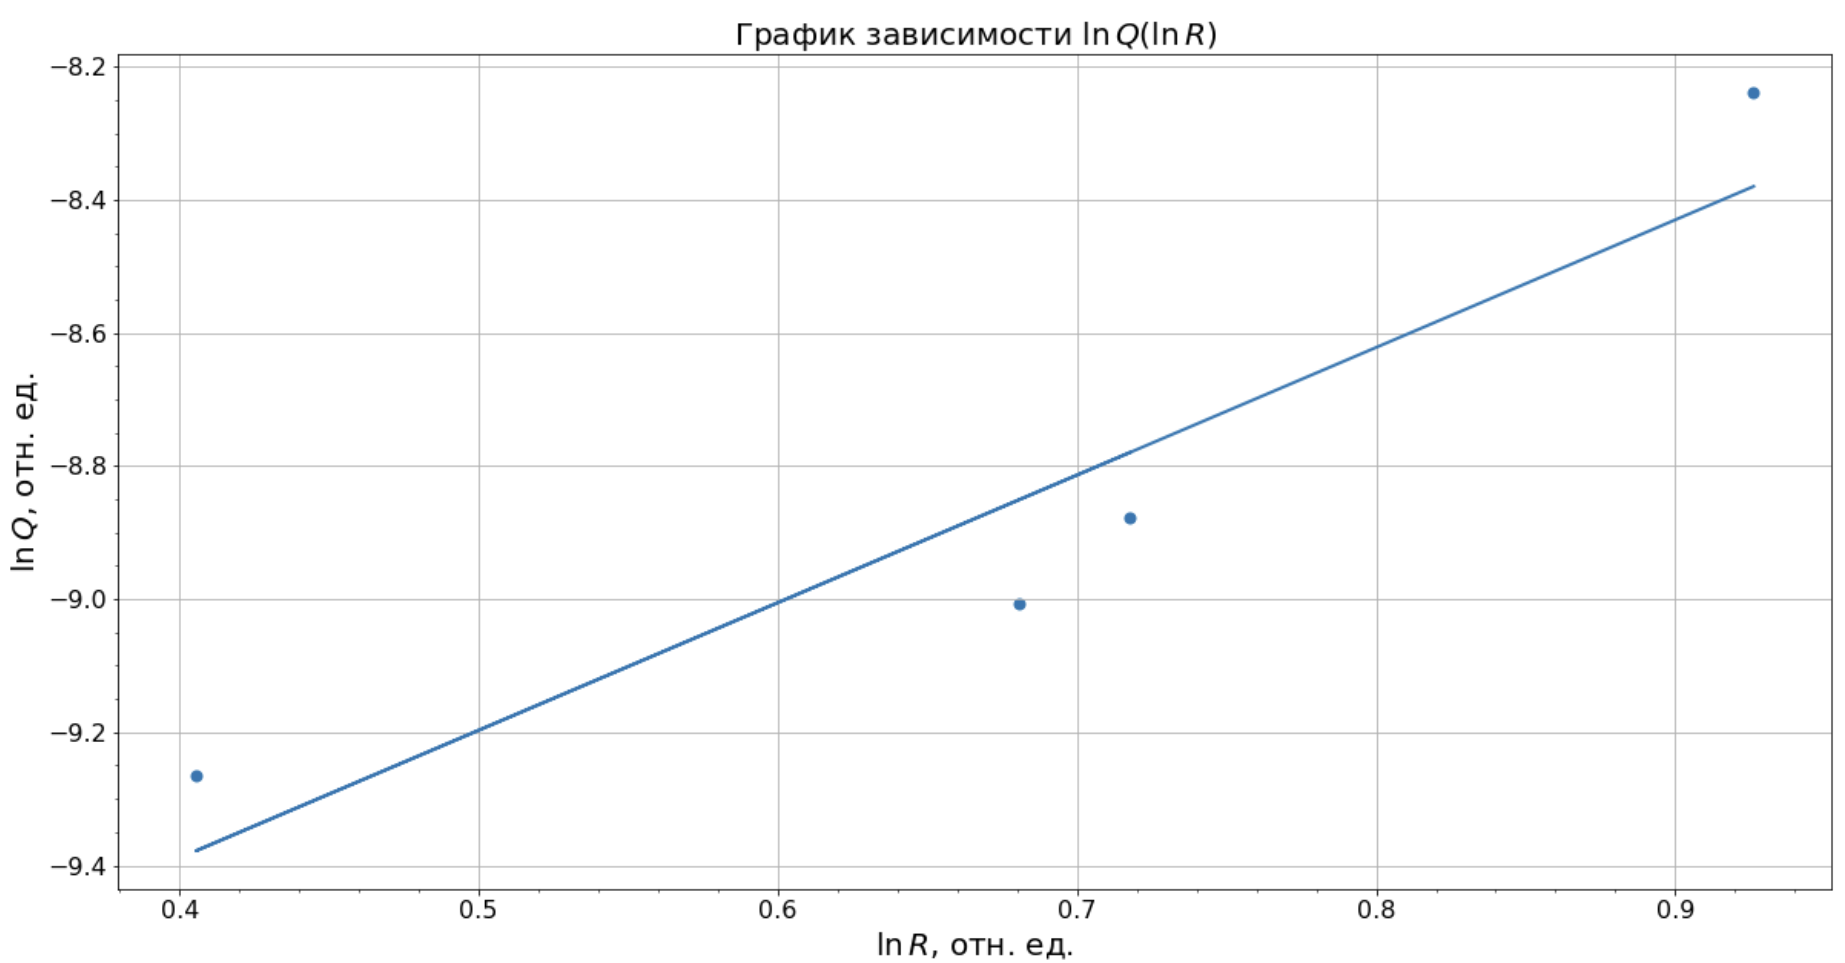
\includegraphics[scale = 0.5]{qr unnorm}
		\caption{График зависимости $\ln Q(\ln R)$ для турбулентного течения}
		\label{graph6}
	\end{figure}

	Полученные коэффициенты по графикам: 
	\begin{itemize}
		\item Для ламинарного течения: $\beta_\text{уст} = 3.13\pm0.56$.
		\item Для турбулентного течения: $\beta_\text{тур} = 1.92\pm 0.50$.
	\end{itemize}

	\section{Вывод}
	
	Экспериментально исследовались свойства течения газов по тонким трубкам при различных числах Рейнольдса; выявить область применимости закона Пуазейля и с его помощью
	определить коэффициент вязкости воздуха. Получили вязкость воздуха:
	\begin{equation*}
		\eta = (1.88\pm 0.1)\text{ Па}\cdot\text{с}
	\end{equation*}
	
	Сравнили зависимость расхода при  ламинарном и турбулентном течении в зависимости от радиуса трубы:
	\begin{itemize}
		\item Для ламинарного течения теоретический коэффициент: $\beta = 4$; Экспериментальный: $\beta_{\text{уст}} = 3.16\pm0.56.$
		\item Для турбулентного течения теоретический коэффициент: $\beta = 2.5$; Экспериментальный: $\beta = 1.92\pm0.50.$
	\end{itemize}
	
	
	
	
	
	
	
	
	
	
	
\end{document}
